\documentclass{article}
\usepackage{amsmath}
\usepackage{amssymb}
\usepackage{graphicx}
\usepackage{hyperref}
\usepackage[version=4]{mhchem}

\title{Example 14}
\date{}

\begin{document}
\maketitle

As shown in the figure, \(A C\) and \(B D\) are two diagonals of trapezoid \(A B C D\) and \(A C \perp B D\). Show that \(A C^{2}+B D^{2}=(A B+D C)^{2}\).

Solution:
Draw \(D A^{\prime} / / C A\) and meets the extension of \(B A\) at \(A\).\\
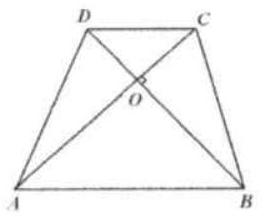
\includegraphics[width=\textwidth]{images/problem_image_1.jpg} \(A^{\prime} A C D\) is a parallelogram with \(A^{\prime} D / / A C\) and \(A^{\prime} D=A C\). Therefore, we know that \(\angle A^{\prime} D B\) is a right angle.\\
\(A^{\prime} D^{2}+D B^{2}=A^{\prime} B^{2} \Rightarrow\)\\
\(A C^{2}+B D^{2}=\left(A^{\prime} A+A B\right)^{2}=(D C+A B)^{2}\)\\
\centering
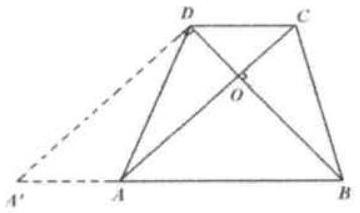
\includegraphics[width=\textwidth]{images/reasoning_image_1.jpg}


\end{document}
